\chapter{Estado del arte}
\label{cap:capitulo2}
En este capítulo se expone el estado del arte de los robots industriales en educación. Esta fase fundamental de la 
investigación se ha completado gracias a la búsqueda en diversas fuentes de renombre, con el fin de 
recopilar información que pueda ser de utilidad para desarrollar el presente proyecto de fin de grado. Como resultado, se 
han seleccionado una serie de trabajos relevantes y significativos en la materia, que se procederán a analizar a continuación.
\begin{itemize}
    \item En \cite{KRIMPENIS2020103} se presenta una solución industrial barata para crear un robot capaz de hacer operaciones de mecanizado (fabricación 
    de piezas mediante operaciones de corte). Es llamado Hydra y esta dotado de 6 \ac{DOF}. Tiene un alcace máximo de casi un metro y un 
    peso que ronda los 13 Kg. Pese a todas estas funciones, está fabricado mediante impresión 3D. 
    Además, tiempo después, se publicó la segunda parte de este artículo: \cite{PAPAPASCHOS2020109}. En el cual se aborda el diseño software y de control 
    que se ha desarrollado para controlar dicho brazo. \\
    En base a lo descrito en estos artículos se han extraido los siguientes puntos fuertes del proyecto:
    \begin{itemize}
        \item Tiene una repitividad de ±0.04 mm.
        \item Tiene un espacio de trabajo muy amplio.
        \item Tener más de 3 grados de libertad le permiten alcanzar gran cantidad de puntos con distintas orientaciones.
        \item Según el árticulo, tiene una capacidad de carga máxima de 12 kilogramos. A pesar de esto, se comenta que en la práctica el peso en el 
        extremo del robot debe ser menor a 5 Kg, por lo que su carga útil rondará los 3 Kg para un funcionamiento acceptable. Esto lo sitúa a la par 
        del robot comercial ABB IRB 120\footnote{\url{https://new.abb.com/products/es/3HAC031431-001/irb-120}}  
    \end{itemize}\
    En cambio, tambíen se deben mencionar los siguientes puntos débiles:
    \begin{itemize}
        \item Carece de integración en \ac{ROS}, plataforma de desarrollo de la que se habla en \ref{subsec:ros2}
        \item Su coste en materiales supera los 1000 \euro \xspace por lo que no es lo suficientemente asequible para su uso académico.
        \item Según este artículo, se necesitan 200 horas para poder imprimir y montar el brazo, lo que implica que es costoso en tiempo 
        crear varias unidades y requiere de cierta habilidad para construirlo correctamente.
        \item En este artículo no se proporcionan los ficheros necesarios para poder replicacarlo. Además, se menciona que las piezas han sido 
        diseñadas mediante el software privativo SolidWorks\textsuperscript{\tiny\textregistered} por lo que lo hace más dificil y costoso de editar.
    \end{itemize}\
    \begin{figure} [h!]
        \begin{center}
          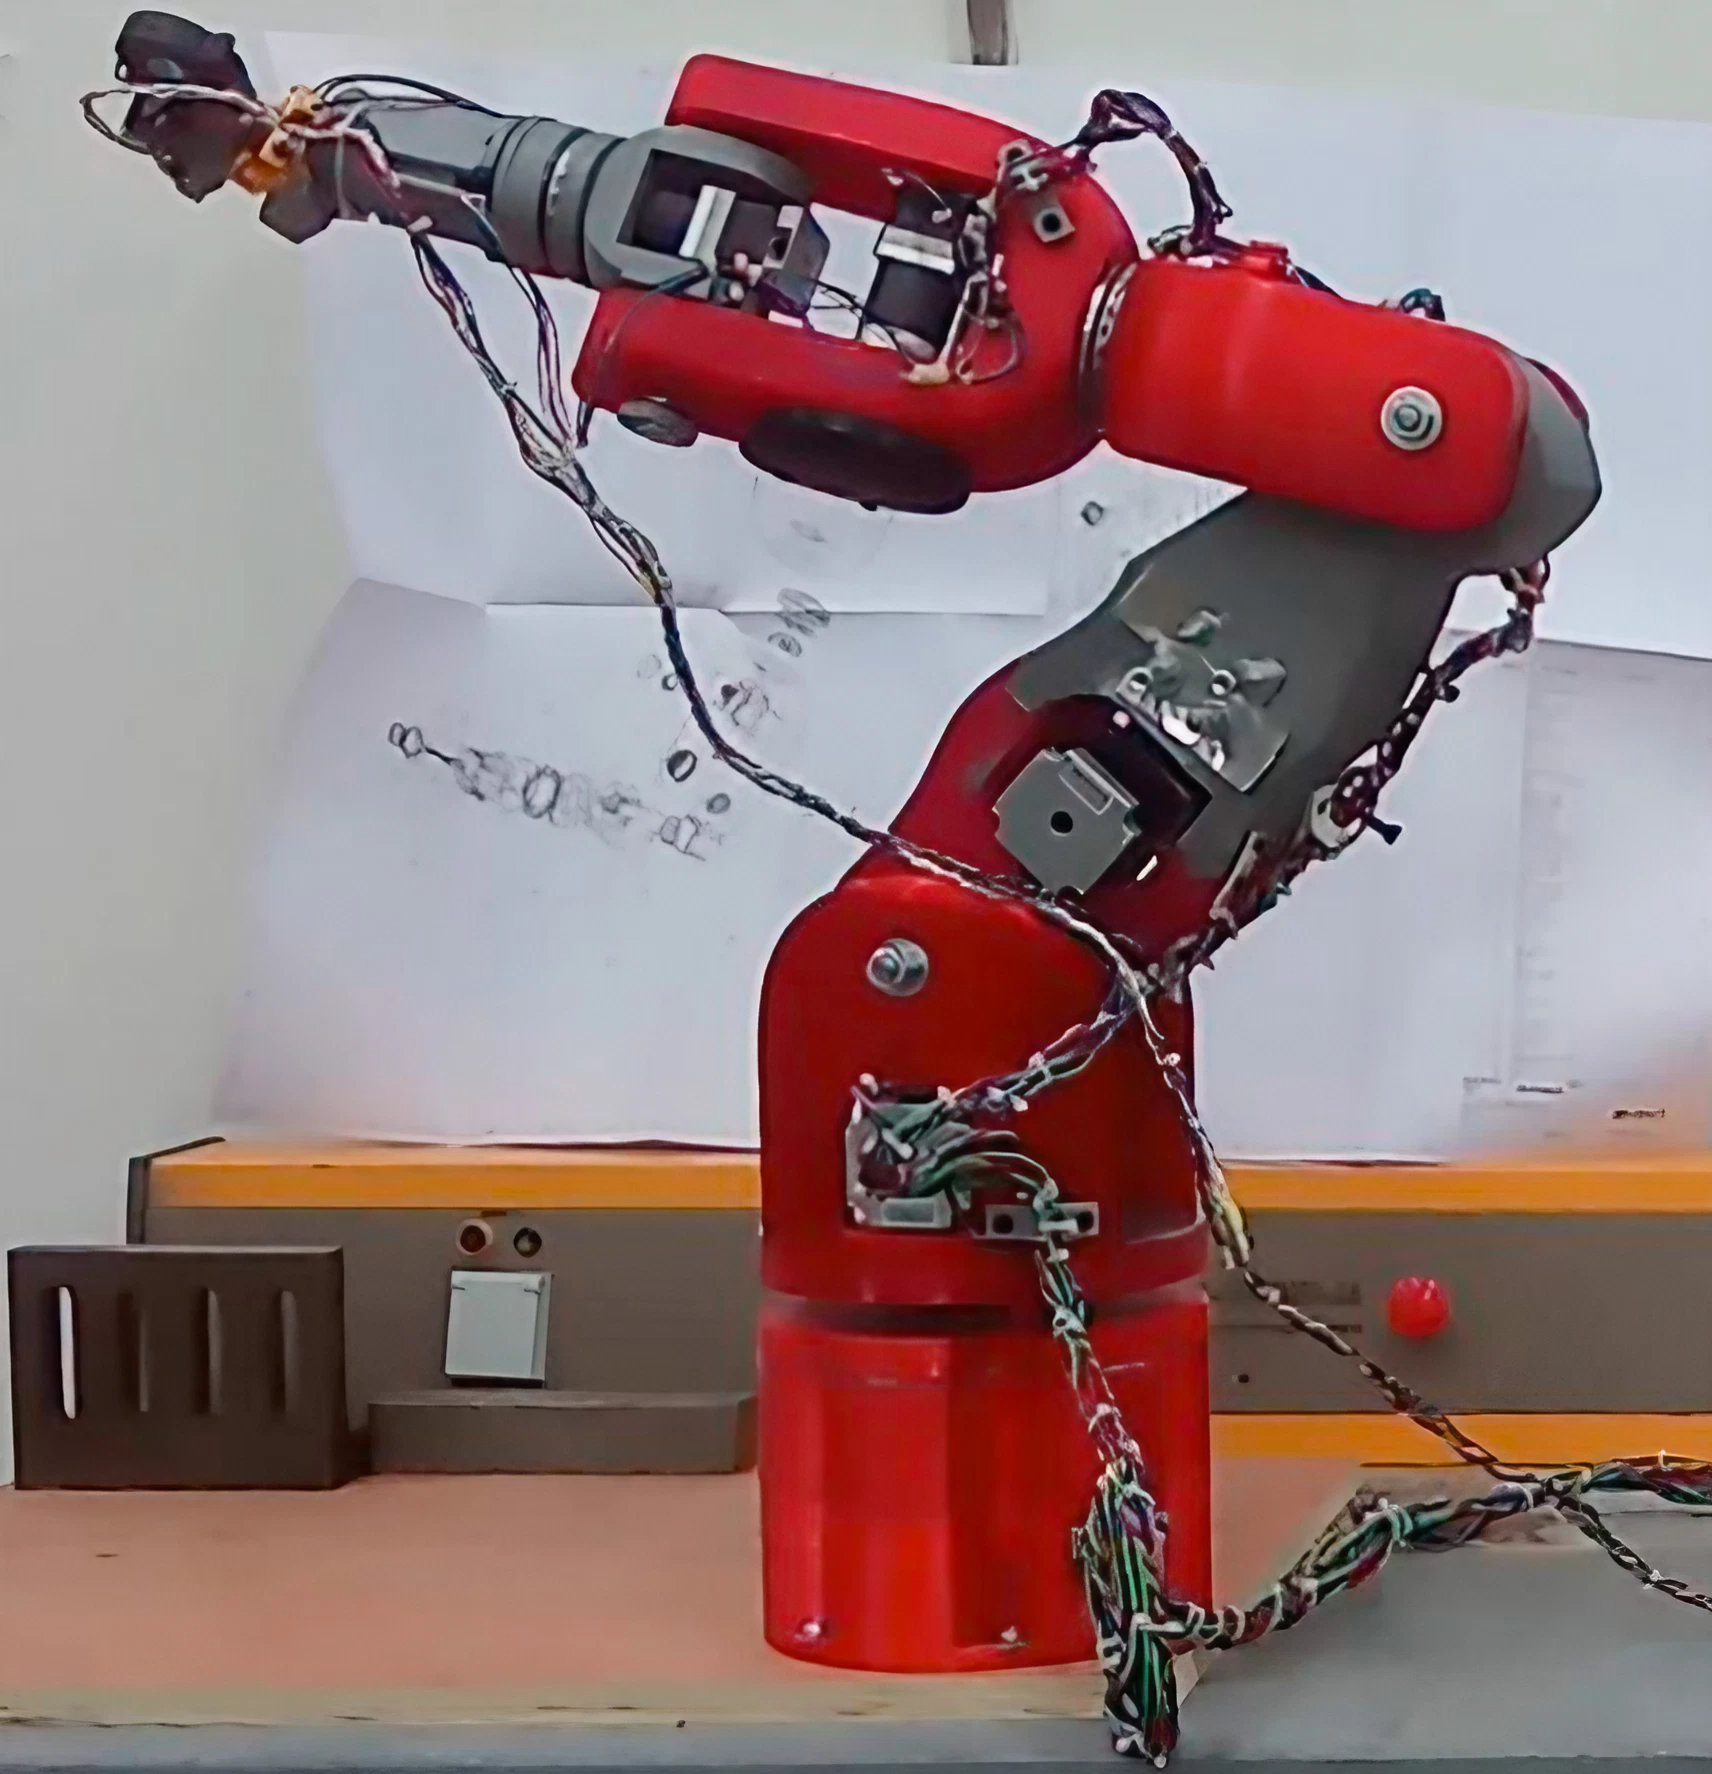
\includegraphics[width=6cm]{figs/Hydra.png}
        \end{center}
        \caption{Robot HydraX}
        \label{fig:hydra}
    \end{figure}\ 
    \item Existen soluciones más sencillas y reproducibles, como por ejemplo la presentada en \cite{adediran2023uiarm}. Se trata de un brazo robótico 
    cuyo propósito es separar botellas de plástico en un proceso de reciclaje. Más allá de la aplicación que se le pretende dar, presentan 
    un manipulador con 4 \ac{DOF} impreso en 3D, de un tamaño menor al anterior. 
    A partir de la información proporcionada en este artículo, se han extraido los siguientes puntos fuertes:
    \begin{itemize}
        \item El diseño de las piezas se ha realizado mediante el uso de la herramienta de diseño FreeCad, esto supone una ventaja respecto 
        a \cite{KRIMPENIS2020103}, que utilizaba una herramienta privativa.
        \item Utiliza motores de pequeño tamaño con una reductora integrada, lo que aumenta su torque y abarata en gran medida los costes 
        del robot. Al haber reducido el consumo de energía, se emplea una electrónica compacta y menos costosa.
        \item Al estar compuesto por menos piezas y tener menos grados de libertad, se demora menos tiempo en imprimir y contruir este robot.
    \end{itemize}\
    Cabe destacar los siguientes puntos negativos:
    \begin{itemize}
        \item El espacio de trabajo (puntos del espacio alcanzables por el extremo del brazo) del robot es demasiado reducido. Esto es debido 
        a la disposición de los grados de libertad. Utiliza dos de ellos para cambiar la orientación del extremo del robot, dejando solo dos para el 
        posicionamiento, por lo que es imposible en la práctica abarcar todo el espacio 3D al alcance del brazo.
        \item Utiliza engranajes impresos en 3D para rotar la segunda articulación comenzando desde la base. Debido a esto, pierde exactitud en función 
        de la posición del brazo debido a la holgura de este tipo de transmisión.
        \item Carece de integración con \ac{ROS} y no proporciona otro tipo de software que permita desarrollar programas para este robot perjudicando la 
        continuidad del proyecto.
    \end{itemize}\
    \begin{figure} [h!]
        \begin{center}
          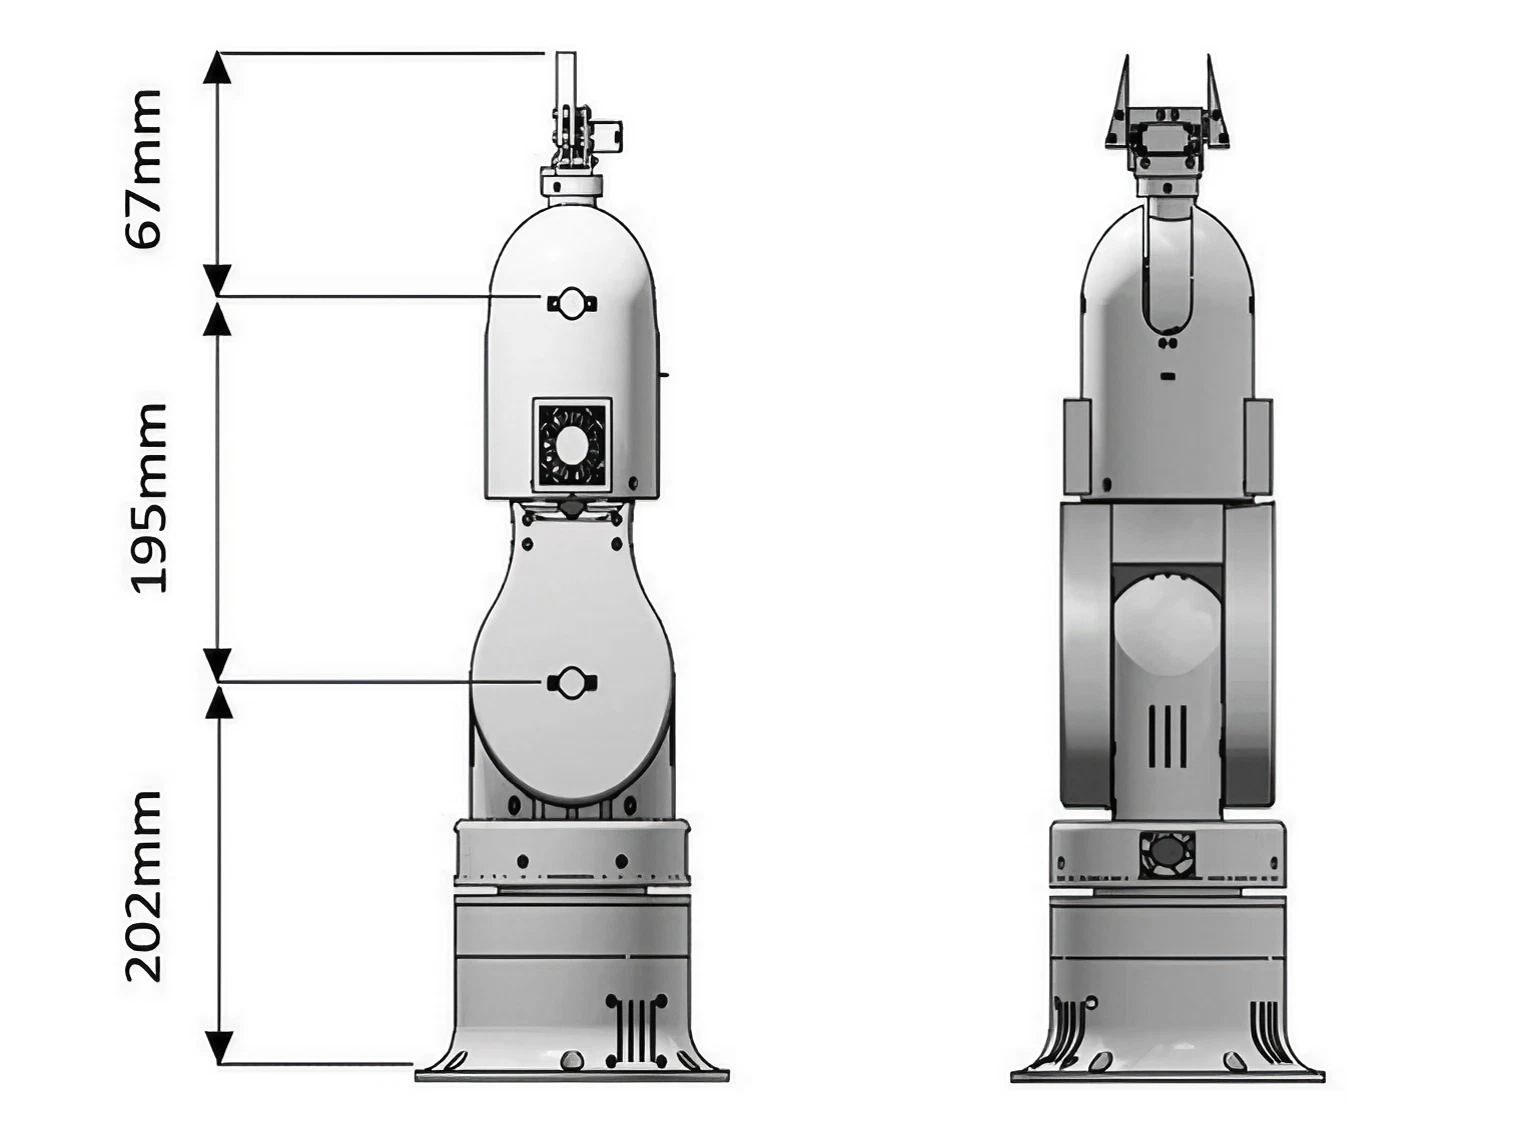
\includegraphics[width=8cm]{figs/uiarm.png}
        \end{center}
        \caption{Robot UIArm}
        \label{fig:uiarm}
    \end{figure}\ 
\end{itemize}\
\vspace{1cm}
